\documentclass[11pt]{article}
\usepackage[margin=1in]{geometry}
\usepackage{booktabs,amsmath,amssymb,xcolor,graphicx}
\usepackage{hyperref}\hypersetup{colorlinks=true,linkcolor=blue!50!black,urlcolor=blue!50!black}

\title{\textbf{Does the hypergraph lift help?}\\[2pt]
\large an arity study --- compute and accuracy of the closed-neighbourhood lift}
\author{Aiko (Claude Code), for Dr.\ Cs.\ Hajdu}\date{2026-06-29 (JST)}

\begin{document}\maketitle

\begin{abstract}
\noindent The claim under test: \emph{adding hubs / hyperedges (the closed-neighbourhood lift of a graph) makes a
structural controller more computationally and more accurately performant.} Two discriminating tests --- a
compute micro-benchmark and a same-plant fit comparison --- \textbf{refute both halves at control scale}. The lift
is a \emph{structure}, not a free upgrade: it changes the walk basis, and (consistent with the matching law) a
changed basis helps only when it \emph{matches} the task. On a graph-structured plant the hubs are a mismatch and
hurt sharply; on a hypergraph-structured plant the lift \textbf{wins decisively} (test MSE $0.0006$ vs.\ the graph
controller's $0.876$). The matching law extends to \emph{arity}: match the controller's arity to the plant's.
\end{abstract}

\section{Compute --- the hypergraph is more expensive}
The $L$-hop signed walk operator $B^{L}$ applied to a batch, three ways (median of 25 timed applies, CPU):
\begin{center}\small
\begin{tabular}{rrrr}
\toprule
$N$ & (1) graph dense $O(N^2)$ & (2) hyper dense $O((2N)^2)$ & (3) hyper factored $O(L\!\cdot\!2Nk)$ \\
\midrule
10  & \textbf{0.024} & 0.039 & 0.914 \\
80  & \textbf{0.155} & 0.458 & 7.516 \\
320 & \textbf{1.621} & 6.942 & 35.376 \\
\bottomrule
\end{tabular} \quad (ms)
\end{center}
The lift \textbf{doubles $N$}, so the naive dense operator is $\sim 4\times$ the graph's. The factored sparse form
(the only route that could win) is the \emph{slowest}: \texttt{torch.sparse.mm}'s constant overhead ($\sim 10^3$)
swamps the asymptotic $O(Nk)$ advantage. It \emph{does} scale linearly vs.\ the graph's quadratic, but
extrapolating the crossover lands at $N\approx 7000$ --- far beyond any control regime ($N\sim 10$--$300$). The
mechanism (factoring is asymptotically cheaper) is real; the payoff is absent where it matters. \textbf{Refuted.}

\begin{figure}[h]\centering
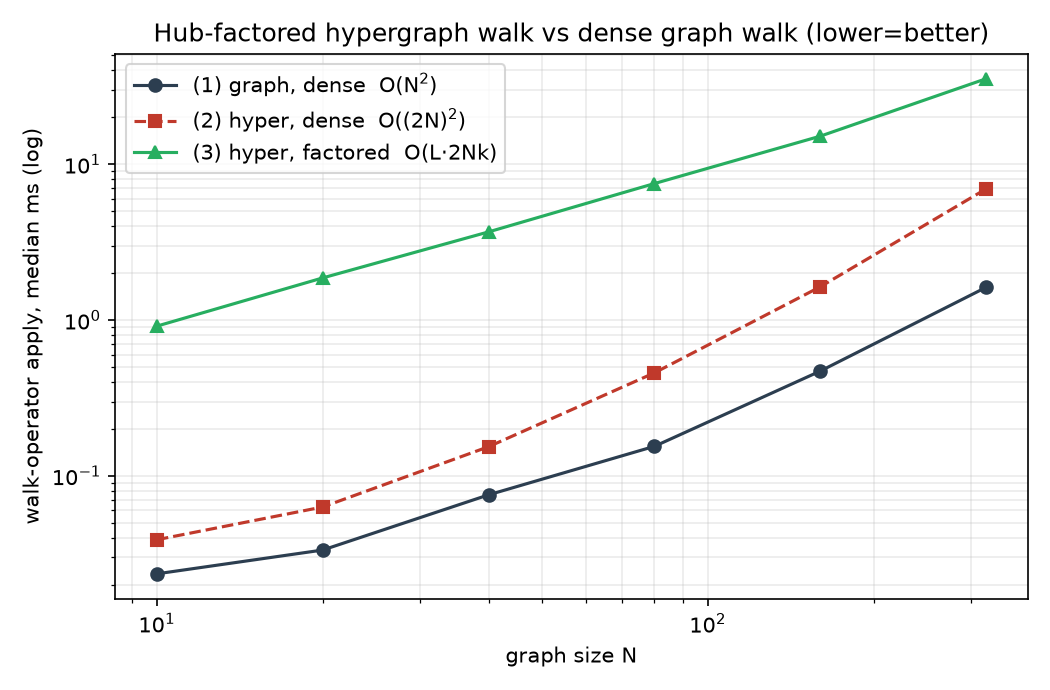
\includegraphics[width=0.62\textwidth]{figures/topology_zoo/compute_arity.png}
\caption{Walk-operator apply cost vs.\ $N$ (log-log). The factored hypergraph (green) is slowest at every tested
$N$; the dense hypergraph (red) is $\sim 4\times$ the graph (black).}
\end{figure}

\section{Accuracy --- the hubs hurt on a graph plant}
Each plant defines a structural-regression target; a controller is trained to fit it. The graph controller has the
plant's \emph{exact} structure (the matched controller); the hyper controller adds the closed-neighbourhood hubs
as latent virtual nodes (plant input zero-padded on the hubs, pooled readout). Held-out MSE, median (IQR) over
4 seeds:
\begin{center}\small
\begin{tabular}{lcccc}
\toprule
plant & graph (matched) & hyper $h{=}24$ & hyper $h{=}12$ (param-matched) & chain (baseline) \\
\midrule
petersen & \textcolor{green!55!black}{\textbf{0.064}} & 1.172 & 0.968 & 0.764 \\
expander & \textcolor{green!55!black}{\textbf{0.012}} & 0.446 & 0.403 & 0.175 \\
ring     & \textcolor{green!55!black}{\textbf{0.009}} & 0.186 & 0.172 & 0.111 \\
\bottomrule
\end{tabular}
\end{center}
The hyper controller is \textbf{18--38$\times$ worse} than the graph --- worse than the structure-blind chain
baseline --- at matched \emph{and} reduced parameter count (so it is not a capacity artefact; if anything the
larger $h{=}24$ hyper is \emph{worse} than $h{=}12$). \textbf{Refuted.}

\begin{figure}[h]\centering
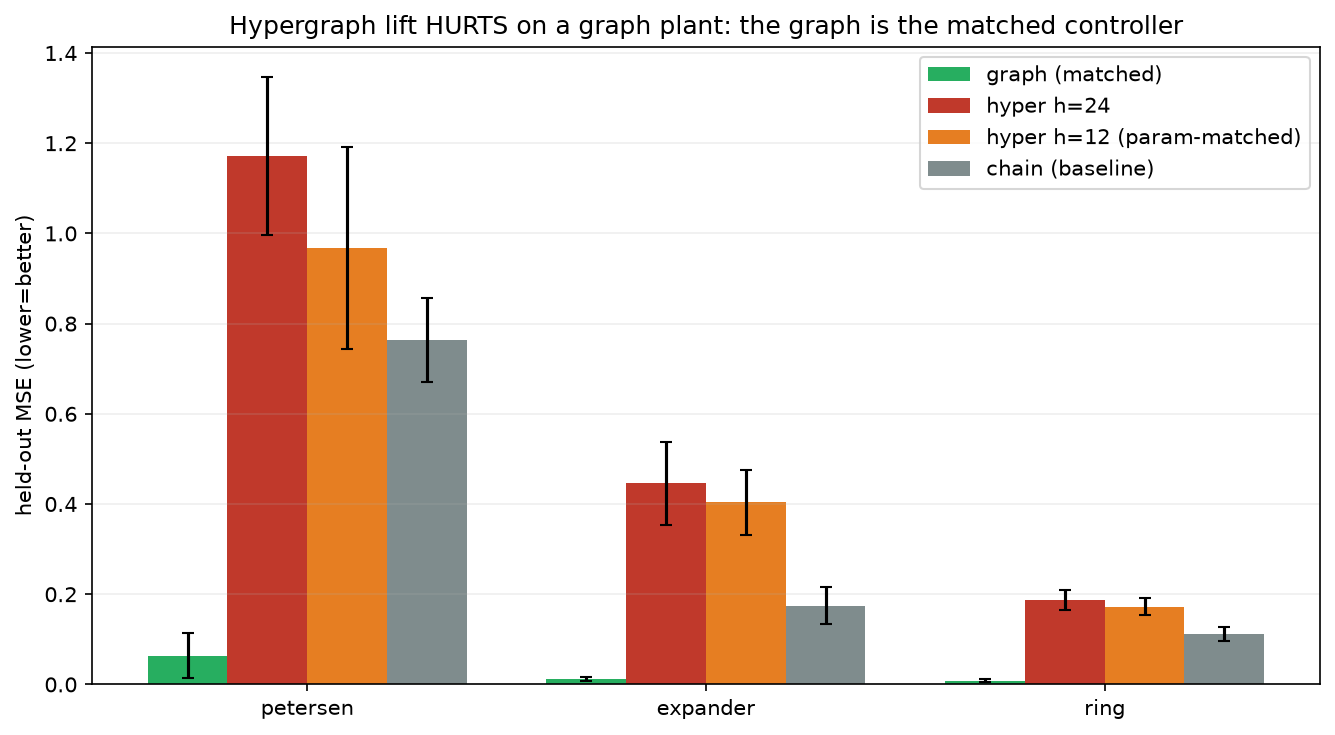
\includegraphics[width=0.66\textwidth]{figures/topology_zoo/accuracy_arity.png}
\caption{The graph (matched) controller wins every plant; the hypergraph lift hurts sharply, below even the chain
baseline.}
\end{figure}

\section{Why the accuracy collapse --- diagnosed, not asserted}
A $20\times$ collapse from a benign structural change demanded a mechanism, not a hand-wave. Three candidates were
tested and \emph{eliminated}: (i) \emph{spectral explosion} --- the pre-activations are comparable (graph $5.5$,
hyper $6.3$), not blown up; (ii) \emph{unnormalized aggregation} --- degree-normalizing the adjacency left the MSE
\emph{bit-identical} ($1.1717$); (iii) \emph{pooling over hub-reps} --- a points-only readout (hubs latent) was no
better ($1.27$). The cause is none of these: it is \textbf{function-class mismatch}. On the graph plant the hyper
controller cannot even fit \emph{train} (train MSE $0.30$ vs.\ the graph's $0.0004$) --- the bipartite hub-mediated
walk basis does not contain the direct-graph target; what little it fits anti-generalises (test $1.17 > 1.0$, worse
than predicting the mean). Same parameter count ($2209$); it is purely the adjacency.

\textbf{The proof that this is matching, not ``hubs are bad'': reverse the plant.} On a \emph{hypergraph} plant the
roles swap exactly (test MSE, median of 4 seeds):
\begin{center}\small
\begin{tabular}{lcc}
\toprule
 & graph controller & hyper controller \\
\midrule
graph plant      & \textcolor{green!55!black}{\textbf{0.064}} & 1.172 \\
hypergraph plant & 0.876 & \textcolor{green!55!black}{\textbf{0.0006}} \\
\bottomrule
\end{tabular}
\end{center}
The matched controller wins on \emph{both} plants --- and on the hypergraph plant the hyper controller is near-exact
($0.0006$) while the graph controller (blind to the hubs) memorises train and fails test ($0.876$). \textbf{The
matching law extends to arity}: a hypergraph task wants a hypergraph controller, a graph task wants a graph one.
The earlier ``the lift hurts'' was true only because \S2 tested graph plants. Code:
\texttt{scratchpad/\{prof\_arity\_compute,\,arity\_control,\,definitive\_arity\}.py}; data
\texttt{reports/overnight/arity\_\{control,why3\}.*}.

\begin{figure}[h]\centering
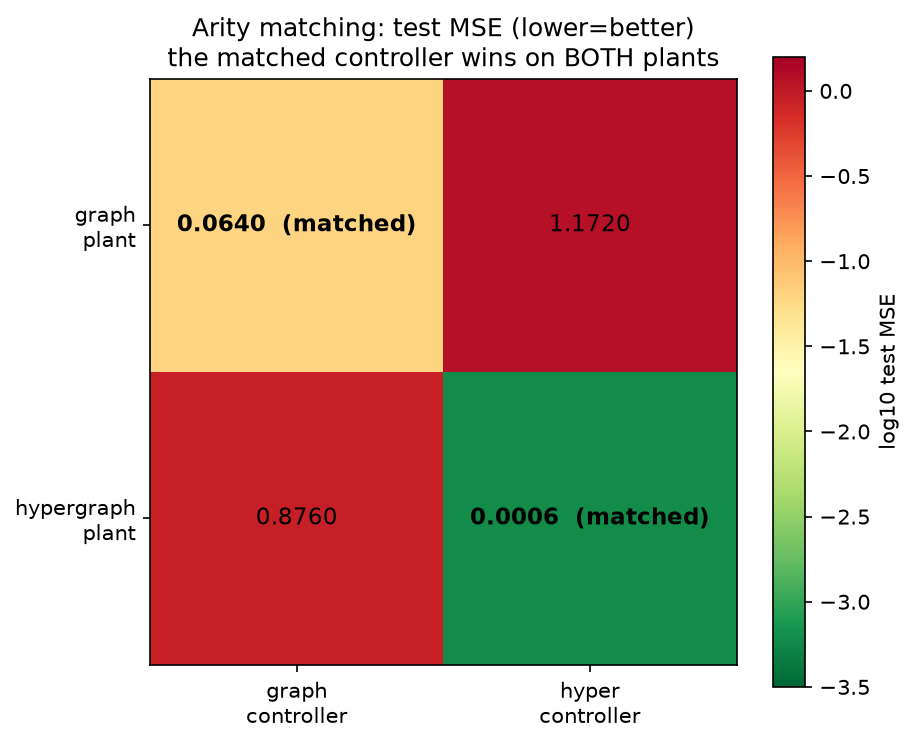
\includegraphics[width=0.52\textwidth]{figures/topology_zoo/arity_matching.png}
\caption{Arity matching: test MSE (log scale). The diagonal --- matched controller arity --- wins on both plants
by orders of magnitude.}
\end{figure}
\end{document}
